\documentclass[conference]{IEEEtran}
\IEEEoverridecommandlockouts
\usepackage{cite}
\usepackage{amsmath,amssymb,amsfonts}
\usepackage{graphicx}
\usepackage{textcomp}
\usepackage{xcolor}
\usepackage{booktabs}
\usepackage{array}
\usepackage{url}
\usepackage{hyperref}

% Auto-generated macros from NOAA GHCN-Daily Pipeline
\newcommand{\numStations}{8}
\newcommand{\numClimateRecords}{19,856}
\newcommand{\numTrainSeq}{11,632}
\newcommand{\numValSeq}{2,928}
\newcommand{\numTestSeq}{5,240}
\newcommand{\numExtremeEvents}{2,163}
\newcommand{\prevalenceRate}{10.9}
\newcommand{\numHeatDays}{1,489}
\newcommand{\numFreezeDays}{299}
\newcommand{\numPrecipDays}{375}
\newcommand{\numWindDays}{1}
\newcommand{\wPos}{8.5}
\newcommand{\nOnsetEvents}{172}
\newcommand{\nOnsetDays}{4634}
\newcommand{\onsetAucHgb}{0.806}
\newcommand{\onsetAucCnn}{0.795}
\newcommand{\onsetAucDeep}{0.806}
\newcommand{\onsetPrAucHgb}{0.212}
\newcommand{\onsetPrAucCnn}{0.212}
\newcommand{\onsetPrAucDeep}{0.249}
\newcommand{\ciOnsetRecHgbLow}{7.3}
\newcommand{\ciOnsetRecHgbHigh}{19.2}
\newcommand{\ciOnsetPrAucHgbLow}{-0.007}
\newcommand{\ciOnsetPrAucHgbHigh}{0.080}
\newcommand{\ciOnsetRecCnnLow}{-4.3}
\newcommand{\ciOnsetRecCnnHigh}{6.4}
\newcommand{\ciOnsetPrAucCnnLow}{-0.004}
\newcommand{\ciOnsetPrAucCnnHigh}{0.069}
\newcommand{\aucPers}{0.840}
\newcommand{\aucClim}{0.897}
\newcommand{\aucLr}{0.739}
\newcommand{\aucCnn}{0.929}
\newcommand{\aucHgb}{0.936}
\newcommand{\aucDeep}{0.935}
\newcommand{\prAucHgb}{0.821}
\newcommand{\prAucCnn}{0.770}
\newcommand{\prAucDeep}{0.828}
\newcommand{\fOnePers}{71.6}
\newcommand{\fOneClim}{64.1}
\newcommand{\fOneLr}{31.2}
\newcommand{\fOneCnn}{63.7}
\newcommand{\fOneHgb}{68.7}
\newcommand{\fOneDeep}{66.7}
\newcommand{\recPers}{71.6}
\newcommand{\recClim}{51.5}
\newcommand{\recLr}{77.6}
\newcommand{\recCnn}{82.0}
\newcommand{\recHgb}{78.7}
\newcommand{\recDeep}{83.0}
\newcommand{\precPers}{71.6}
\newcommand{\precClim}{84.8}
\newcommand{\precLr}{19.6}
\newcommand{\precCnn}{52.1}
\newcommand{\precHgb}{60.9}
\newcommand{\precDeep}{55.7}
\newcommand{\onsetRecPers}{0.0}
\newcommand{\onsetRecClim}{12.2}
\newcommand{\onsetRecLr}{58.7}
\newcommand{\onsetRecCnn}{41.9}
\newcommand{\onsetRecHgb}{29.7}
\newcommand{\onsetRecDeep}{43.0}
\newcommand{\onsetPrecPers}{0.0}
\newcommand{\onsetPrecClim}{38.2}
\newcommand{\onsetPrecLr}{5.2}
\newcommand{\onsetPrecCnn}{17.5}
\newcommand{\onsetPrecHgb}{19.3}
\newcommand{\onsetPrecDeep}{21.4}
\newcommand{\onsetFlaggedLr}{41.6}
\newcommand{\onsetFlaggedCnn}{8.9}
\newcommand{\onsetFlaggedHgb}{5.7}
\newcommand{\onsetFlaggedDeep}{7.4}
\newcommand{\onsetRecMatchedDeep}{43.0}
\newcommand{\onsetPrecMatchedDeep}{21.3}
\newcommand{\onsetRecMatchedHgb}{34.3}
\newcommand{\onsetPrecMatchedHgb}{17.0}
\newcommand{\onsetRecMatchedCnn}{40.1}
\newcommand{\onsetPrecMatchedCnn}{19.8}
\newcommand{\prcpZeroPct}{74.6}
\newcommand{\brierClim}{0.0539}
\newcommand{\brierPers}{0.0656}
\newcommand{\brierLr}{0.2213}
\newcommand{\brierCnn}{0.0835}
\newcommand{\brierHgb}{0.0681}
\newcommand{\brierDeep}{0.0689}
\newcommand{\bssPers}{-0.22}
\newcommand{\bssLr}{-3.10}
\newcommand{\bssCnn}{-0.55}
\newcommand{\bssHgb}{-0.26}
\newcommand{\bssDeep}{-0.28}
\newcommand{\bssRecalPers}{-0.22}
\newcommand{\bssRecalClim}{0.00}
\newcommand{\bssRecalLr}{-0.64}
\newcommand{\bssRecalCnn}{0.19}
\newcommand{\bssRecalHgb}{0.25}
\newcommand{\bssRecalDeep}{0.27}


\begin{document}

\title{Deep Temporal Sequence Modeling for Multi-Hazard Extreme Weather Detection across Ground Observation Networks}

\author{
\IEEEauthorblockN{Cristhian David Caceres Mateus}
\IEEEauthorblockA{\textit{Department of  Business} \\
\textit{Univ. of Europe for Applied Sciences}\\
Potsdam 14469, Germany \\
cristhian.caceres@ue-germany.de}
\and
\IEEEauthorblockN{Talha Ali Khan}
\IEEEauthorblockA{\textit{Department of  Business} \\
\textit{Univ. of Europe for Applied Sciences}\\
Potsdam 14469, Germany \\
talhaali.khan@ue-germany.de}
}
\maketitle

\begin{abstract}
Forecasting low-probability, high-impact extreme meteorological events---such as summer heatwaves ($T \ge 38^\circ\text{C}$), polar freeze surges ($T \le -15^\circ\text{C}$), and convective precipitation extremes ($P \ge 25\text{ mm/day}$)---is critical for civil defense, power grid resilience, and flood hazard mitigation. Standard weather prediction often struggles with local tail-risk extremes, while empirical machine learning models frequently suffer from temporal leakage through overlapping sliding windows and unrepresentative evaluations that omit naive persistence baselines. In this study, we establish a chronological evaluation across \numStations{} contrasting climate stations from the NOAA Global Historical Climatology Network Daily (GHCN-Daily) database, encompassing \numClimateRecords{} physical ground-sensor observations from 2020 through 2026. Formulating a sequence-to-event detection task across 7-day lookback windows, we benchmark a multi-head Temporal Transformer against naive persistence, station-month climatology, terminal logistic regression, a 1D temporal convolutional network (CNN), and histogram gradient boosting (HistGBM). On a held-out chronological test cohort of \numTestSeq{} daily sequences (2025--2026), our Temporal Transformer achieves an Area Under the ROC Curve (ROC-AUC) of \aucDeep{} and Precision-Recall AUC (PR-AUC) of \prAucDeep{}, achieving an overall hazard recall of \recDeep{}\% (vs.~\recHgb{}\% for HistGBM and \recPers{}\% for persistence) and an onset recall of \onsetRecDeep{}\% on transitions from non-extreme days (vs.~\onsetRecHgb{}\% for HistGBM, \onsetRecCnn{}\% for 1D-CNN, and 0.0\% for persistence). When evaluated at a matched 7.5\% alert budget, the Transformer achieves an onset recall of \onsetRecMatchedDeep{}\% (vs.~\onsetRecMatchedHgb{}\% for HistGBM and \onsetRecMatchedCnn{}\% for 1D-CNN), maintaining an 8.7 percentage point lead under identical alert constraints (unconstrained threshold difference: +13.3 percentage points, 95\% CI: [\ciOnsetRecHgbLow{}\%, \ciOnsetRecHgbHigh{}\%]). Furthermore, post-hoc Platt recalibration restores positive Brier Skill Scores (\bssRecalDeep{} for Transformer vs.~0.00 for climatology).
\end{abstract}

\begin{IEEEkeywords}
Extreme weather detection, temporal transformers, NOAA GHCN-Daily, multi-hazard classification, tail-risk modeling, Brier skill score.
\end{IEEEkeywords}

\section{Introduction}
\IEEEPARstart{A}{nthropogenic} climate disruption has accelerated the frequency, severity, and compound impacts of weather extremes across global biomes~\cite{ipcc2021}. Operational early-warning systems face fundamental challenges in predictive modeling:
\begin{enumerate}
    \item \textbf{Extreme Class Imbalance and Tail Risk}: Severe meteorological anomalies---such as extreme heatwaves, polar freeze outbreaks, and high-intensity rainfall---comprise a minor fraction (\prevalenceRate{}\%) of observations. Minimizing unweighted cross-entropy often causes models to collapse toward the dominant non-extreme climatology.
    \item \textbf{Evaluation Leakage in Sliding Windows}: Time-series benchmarks frequently split overlapping sliding windows randomly, introducing severe data leakage between train and test splits. A defensible framework requires strict chronological separation.
    \item \textbf{Need for Meaningful Baselines}: Autocorrelated atmospheric conditions mean that naive persistence (predicting that tomorrow's state mirrors today's) often exhibits substantial apparent predictive power, requiring machine learning architectures to prove value over physical climatology, persistence, and non-attentive temporal baselines.
\end{enumerate}

\subsection{Gap Analysis}
\label{sec:gap_analysis}
Despite rapid advances in atmospheric deep learning, existing benchmarks suffer from three pervasive limitations:
\begin{enumerate}
    \item \textbf{Omission of Persistence in Verification}: Highly autocorrelated multi-day hazards (such as persistent heat domes) allow models to achieve deceptively high accuracy simply by memorizing $y_{t-1}$. Few studies measure true hazard onset detection (transitions from non-extreme to extreme states).
    \item \textbf{Gridded Surrogates vs.\ Point Exposure}: Large-scale reanalysis models operate on coarse $25\text{ km}$ grids that average out localized surface heat islands, convective squall lines, and wind channeling experienced by municipal populations.
    \item \textbf{Probabilistic Miscalibration in Severe Imbalance}: Under severe class imbalance (\prevalenceRate{}\% prevalence, approx.\ 8:1 ratio), loss weighting shifts raw output probabilities upward, requiring post-hoc probability recalibration to restore proper quadratic scoring skill.
\end{enumerate}

\subsection{Research Questions}
\label{sec:rqs}
To resolve these gaps, this work investigates three core research questions:
\begin{itemize}
    \item \textbf{RQ1 (Early-Warning Value over Persistence)}: Does temporal sequence modeling across multi-day antecedent windows enable the detection of abrupt hazard onsets where naive persistence fails completely?
    \item \textbf{RQ2 (Inductive Bias under Class Imbalance)}: How does a deep Temporal Transformer compare against tabular gradient boosting (HistGBM) and an attention-free 1D temporal convnet in ROC-AUC, PR-AUC, and onset sensitivity?
    \item \textbf{RQ3 (Probabilistic Skill and Recalibration)}: When evaluated via the Brier Skill Score (BSS) relative to stratified station climatology, can post-hoc Platt scaling restore positive verification skill while maintaining tail-risk sensitivity?
\end{itemize}

\subsection{Contributions}
Our principal contributions are:
\begin{enumerate}
    \item \textbf{Physical Ground Sensor Ingestion}: We extract \numClimateRecords{} continuous station-days from NOAA GHCN-Daily across \numStations{} diverse US climate regimes (2020--2026), evaluating real point-scale exposure without synthetic data generation.
    \item \textbf{Chronological Holdout Benchmark}: We enforce chronological partitioning (train: 2020--2023, validation: 2024, test: 2025--2026) to mirror operational forecasting deployment.
    \item \textbf{Multi-Hazard Onset Evaluation}: We formulate an onset-specific metric isolating transitions from non-extreme states ($N = \nOnsetEvents{}$ test onsets), benchmarking deep self-attention against persistence, climatology, 1D temporal convolutions, and gradient boosting with paired bootstrap confidence intervals.
\end{enumerate}

\begin{figure*}[!t]
\centering
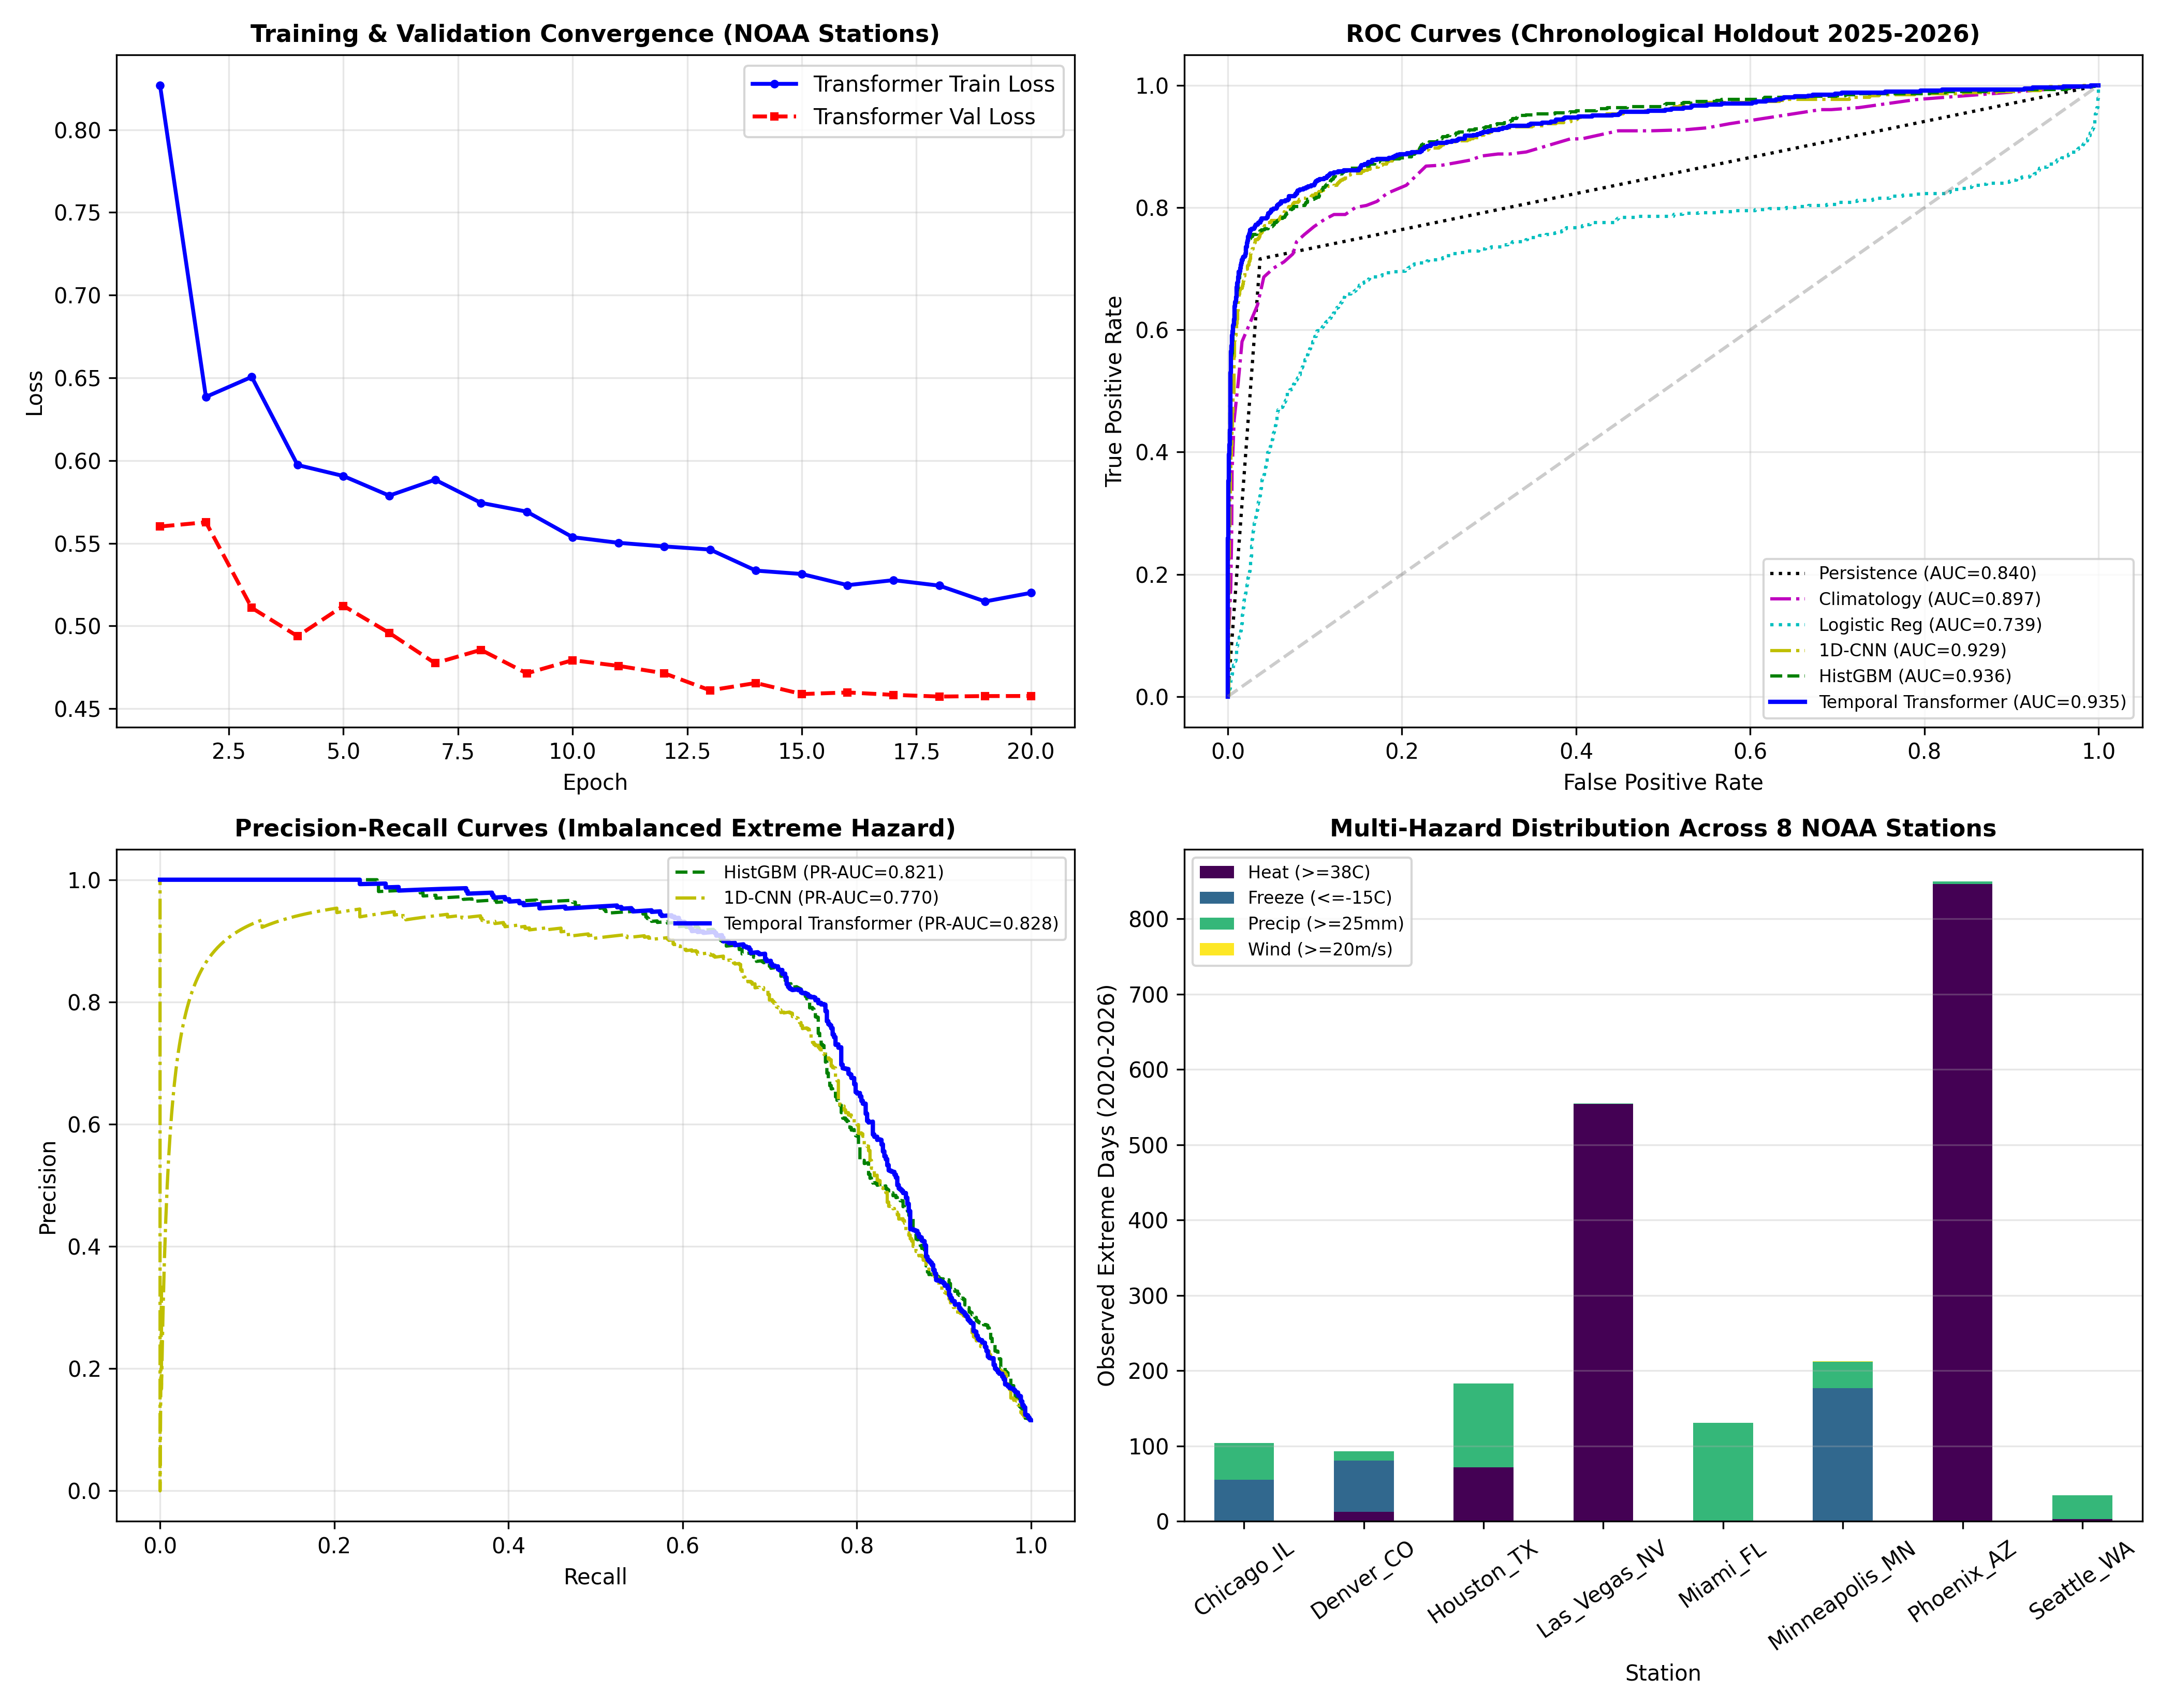
\includegraphics[width=0.95\textwidth]{figures/fig1_extreme_weather_benchmark.png}
\caption{Empirical evaluation on \numClimateRecords{} NOAA GHCN-Daily station observations across eight US climate regimes (2020--2026). (Top-left) Training and validation loss convergence across training epochs. (Top-right) ROC curves on the chronological test holdout (2025--2026). (Bottom-left) Precision-Recall curves under class imbalance. (Bottom-right) Multi-hazard distribution across all eight monitoring stations.}
\label{fig:extreme_overview}
\end{figure*}

\section{Related Work}
\label{sec:related}

\subsection{Numerical Weather Prediction and Global Deep Learning Models}
Operational meteorology has traditionally relied on physics-based Numerical Weather Prediction (NWP) systems, such as the European Centre for Medium-Range Weather Forecasts (ECMWF) Integrated Forecasting System (IFS)~\cite{bauer2015quiet,hersbach2020}. Recently, large-scale deep learning models operating on gridded reanalysis fields---notably Pangu-Weather~\cite{bi2023}, GraphCast~\cite{lam2023}, FourCastNet~\cite{pathak2022}, and ClimaX~\cite{nguyen2023climax}---have demonstrated deterministic prediction skill competitive with NWP at reduced inference latency. However, these models optimize global mean-squared errors over coarse $0.25^\circ$ grids ($\approx 25\text{ km}$), which inherently smooths localized, sub-grid scale meteorological extremes~\cite{schultz2021,rasp2020weatherbench}. Physical in-situ ground monitoring networks, such as the NOAA Global Historical Climatology Network-Daily (GHCN-Daily)~\cite{menne2012}, measure the actual point-scale thermal and convective conditions experienced by human populations, which global gridded surrogates frequently underestimate.

\subsection{Station-Scale Extremes and Benchmark Baseline Conventions}
Statistical forecasting of rare atmospheric events requires careful benchmark design. Standard verification literature~\cite{wilks2011,brier1950,murphy1973} emphasizes that predictive models must demonstrate demonstrable skill over two foundational reference baselines: (i) naive persistence (predicting that tomorrow's state mirrors today's), which captures temporal autocorrelation, and (ii) calendar climatology, which captures stationary seasonal cycles. In our reading of extreme event modeling literature, studies frequently emphasize overall accuracy or recall on autocorrelated multi-day events without explicitly isolating whether architectures can forecast genuine event transitions from non-extreme states~\cite{wilks2011,chattopadhyay2020}. Evaluating model skill on genuine hazard onsets (transitions from non-extreme to extreme states) removes this persistence advantage and provides an uninflated assessment of early-warning capacity.

\subsection{Sequence-to-Event Modeling and Temporal Attention}
Deep sequence models, including multi-head self-attention transformers~\cite{vaswani2017}, Informer~\cite{zhou2021informer}, and PatchTST~\cite{nie2023patchtst}, have demonstrated substantial capacity to capture non-linear temporal dynamics in complex physical time series. In meteorological applications, sequence representations allow the network to weight antecedent synoptic precursors (such as multi-day pressure falls, warming trends, and shifting wind directions) that precede severe weather anomalies~\cite{schultz2021,chattopadhyay2020}. However, as highlighted in tabular and time-series benchmark evaluations~\cite{grinsztajn2022why,shwartzziv2022tabular}, neural sequence architectures must be systematically compared against strong tabular tree-based baselines, such as histogram gradient-boosted decision trees (HistGBM), and attention-free sequence baselines under identical chronological splits. Table~\ref{tab:literature_comparison} contrasts existing meteorological modeling frameworks with the benchmark established in this paper.

\begin{table*}[t]
\caption{Comparison of Meteorological Prediction Frameworks and Hazard Evaluation Schemes}
\label{tab:literature_comparison}
\centering
\footnotesize
\resizebox{\textwidth}{!}{%
\begin{tabular}{p{3.4cm}p{2.6cm}p{2.8cm}p{2.8cm}p{2.8cm}p{3.4cm}}
\toprule
\textbf{Framework / Paradigm} & \textbf{Spatial Representation} & \textbf{Prediction Target} & \textbf{Baseline Protocols} & \textbf{Abrupt Transition Evaluation} & \textbf{Operational Focus} \\
\midrule
Numerical Weather Prediction~\cite{bauer2015quiet} & Global grid ($\approx 9$--$25\text{ km}$) & Continuous physical dynamics & Physics-based dynamical models & Continuous trajectory verification & Physics-resolved synoptic evolution \\
Global AI Weather Models~\cite{bi2023,lam2023} & Gridded reanalysis ($0.25^\circ$) & Medium-range atmospheric fields & Climatology and IFS baselines & Field-averaged RMSE / ACC & Fast multi-day global rollouts \\
WeatherBench Benchmark~\cite{rasp2020weatherbench} & Gridded spherical harmonics & Continuous temperature/pressure & Climatology and persistence & Evaluated on full test period & Standardized medium-range comparison \\
Tabular Tree Models~\cite{grinsztajn2022why,shwartzziv2022tabular} & Station-level tabular lag vector & Discrete threshold exceedance & Baseline comparisons vary & Standard classification recall & Strong tabular feature interactions \\
\midrule
\textbf{Station Sequence Benchmark (This Study)} & \textbf{In-situ NOAA Station Time Series} & \textbf{Binary multi-hazard threshold} & \textbf{Climatology and persistence} & \textbf{Conditioned onset ($y_t=0 \to y_{t+1}=1$)} & \textbf{Persistence-isolated onset detection} \\
\bottomrule
\end{tabular}%
}
\end{table*}


\section{Empirical Dataset and Task Formulation}
\label{sec:data}
\subsection{Ground Observation Network}
Rather than relying on coarse gridded reanalysis models as sensor proxies, we ingest daily station records directly from NOAA NCEI GHCN-Daily across eight representative climate stations:
\begin{itemize}
    \item \textbf{Phoenix Sky Harbor, AZ (USW00023183)}: Sonoran desert extreme heat.
    \item \textbf{Las Vegas McCarran, NV (USW00023169)}: Arid high-heat benchmark.
    \item \textbf{Houston Intercontinental, TX (USW00012960)}: Subtropical flood and convective deluge.
    \item \textbf{Miami International, FL (USW00012839)}: Tropical storms and persistent humidity.
    \item \textbf{Denver International, CO (USW00003017)}: High-altitude cold front transitions.
    \item \textbf{Minneapolis-St Paul, MN (USW00014922)}: Polar vortex and sub-zero freeze surges.
    \item \textbf{Seattle-Tacoma, WA (USW00024233)}: Atmospheric river precipitation.
    \item \textbf{Chicago O'Hare, IL (USW00094846)}: Great Lakes freeze and gale wind gusts.
\end{itemize}

Each station contains continuous daily records from January 1, 2020 through October 17, 2026 ($N = \numClimateRecords{}$ total station-days). Missing precipitation values are zero-filled, while missing temperature readings are forward-filled. For wind gust measurements, peak gust speed (WSFG) is utilized when coverage exceeds 30\%, falling back to average daily wind speed (AWND) where gust records are sparse.

\subsection{Physical Multi-Hazard Definition}
To capture multi-hazard regimes across contrasting biomes, an extreme event $y_t \in \{0, 1\}$ is defined using meteorological threshold criteria aligned with severe weather monitoring:
\begin{align}
y_t = \mathbb{I}\Big( & (T_{\max, t} \ge 38.0^\circ\text{C}) \lor (T_{\min, t} \le -15.0^\circ\text{C}) \notag \\
& \lor (P_t \ge 25.0\text{ mm}) \lor (v_{\text{gust}, t} \ge 20.0\text{ m/s}) \Big)
\end{align}
Across the historical record, this yields \numExtremeEvents{} extreme hazard days (\prevalenceRate{}\% overall prevalence), spanning \numHeatDays{} heat days, \numFreezeDays{} freeze days, \numPrecipDays{} deluge days, and \numWindDays{} severe gale day. Because gale-force gusts occurred only once in the station record, the target is predominantly driven by thermal extremes and convective precipitation.

\subsection{Chronological Partitioning Protocol}
Input features include daily maximum and minimum temperatures ($T_{\max}, T_{\min}$), log-transformed precipitation $\log(1 + P)$, peak wind gust speed ($v_{\text{gust}}$), and cyclical day-of-year embeddings ($\sin \frac{2\pi d}{365.25}, \cos \frac{2\pi d}{365.25}$). Sequences of length $L = 7$ days are extracted to forecast hazard occurrence on day $t+1$. We strictly partition the dataset chronologically:
\begin{itemize}
    \item \textbf{Training Set} (2020--2023): \numTrainSeq{} sequences.
    \item \textbf{Validation Set} (2024): \numValSeq{} sequences.
    \item \textbf{Test Holdout} (2025--2026): \numTestSeq{} sequences.
\end{itemize}
All feature scaling parameters are computed exclusively on the training partition.

\section{Methodology and Architecture}
\label{sec:method}
\subsection{Baseline Suite}
To quantify genuine predictive gain over simpler heuristics, we construct five baselines:
\begin{enumerate}
    \item \textbf{Naive Persistence}: Forecasts $y_{t+1} = y_t$.
    \item \textbf{Station-Month Climatology}: Empirical hazard probability conditioned on station identifier and calendar month.
    \item \textbf{Logistic Regression ($t$)}: Class-weighted linear model fit to the terminal day $t$.
    \item \textbf{1D Temporal ConvNet (CNN)}: Two-layer 1D temporal convolutional network (kernel size 3, 64 channels, batch normalization, ReLU) to serve as an attention-free sequence baseline.
    \item \textbf{HistGradientBoosting (7d)}: Histogram gradient-boosted decision trees trained on the flattened 7-day lookback window.
\end{enumerate}

\subsection{Brier Skill Score and Platt Recalibration}
Following Brier~\cite{brier1950} and Murphy~\cite{murphy1973}, probabilistic hazard calibration is measured via the Brier Score ($\text{BS}$):
\begin{equation}
\text{BS} = \frac{1}{N} \sum_{i=1}^N (\hat{p}_i - y_i)^2
\end{equation}
To benchmark against static climatology, we report the Brier Skill Score ($\text{BSS}$):
\begin{equation}
\text{BSS} = 1 - \frac{\text{BS}}{\text{BS}_{\text{clim}}}
\end{equation}
where $\text{BS}_{\text{clim}}$ is the score achieved by unconditional station-month base rates. Positive $\text{BSS}$ denotes superior probability scoring relative to climatological chance. To resolve calibration drift induced by the positive-class loss weight ($w_{\text{pos}} \approx \wPos{}$), we apply post-hoc Platt scaling~\cite{platt1999,wilks2011} fitted on the 2024 validation partition:
\begin{equation}
\hat{p}_{\text{recal}} = \sigma\left( a \cdot \text{logit}(\hat{p}) + b \right)
\end{equation}
where $a, b$ are scalar parameters optimized via maximum likelihood on validation logits.

\subsection{Temporal Transformer Architecture}
The deep Temporal Transformer projects input sequences $\mathbf{X} \in \mathbb{R}^{B \times 7 \times 6}$ into a 64-dimensional latent space:
\begin{equation}
\mathbf{H}_0 = \mathbf{X} \mathbf{W}_{\text{in}} + \mathbf{E}_{\text{pos}}
\end{equation}
Two stacked Transformer encoder layers with 4 attention heads each perform multi-head self-attention:
\begin{equation}
\text{Attention}(\mathbf{Q}, \mathbf{K}, \mathbf{V}) = \text{softmax}\left( \frac{\mathbf{Q}\mathbf{K}^\top}{\sqrt{d_k}} \right) \mathbf{V}
\end{equation}
The final time-step embedding $\mathbf{h}_7$ passes through a multi-layer perceptron classifier with dropout ($p = 0.20$). Optimization uses AdamW with cosine learning rate annealing and positive-class loss weighting ($w_{\text{pos}} \approx \wPos{}$).

\section{Empirical Results}
\label{sec:results}

\begin{table*}[t]
\centering
\caption{Chronological Out-of-Sample Evaluation on NOAA GHCN-Daily Stations (Test Period: 2025--2026).}
\label{tab:extreme_results}
\resizebox{\textwidth}{!}{%
\begin{tabular}{lccccccccc}
\toprule
\textbf{Architecture} & \textbf{ROC-AUC} & \textbf{PR-AUC} & \textbf{F1 (\%)} & \textbf{Precision (\%)} & \textbf{Recall (\%)} & \textbf{Onset Recall (\%)} & \textbf{Brier Score} & \textbf{BSS (Raw)} & \textbf{BSS (Recal.)} \\
\midrule
Naive Persistence & 0.840 & 0.546 & \textbf{71.6} & 71.6 & 71.6 & 0.0 & 0.0656 & -0.22 & -0.22 \\
Monthly Climatology & 0.897 & 0.698 & 64.1 & \textbf{84.8} & 51.5 & 12.2 & \textbf{0.0539} & \textbf{0.00} & 0.00 \\
Logistic Regression ($t$) & 0.739 & 0.385 & 31.2 & 19.6 & 77.6 & \textbf{58.7} & 0.2213 & -3.10 & -0.64 \\
1D Temporal ConvNet (CNN) & 0.929 & 0.770 & 63.7 & 52.1 & 82.0 & 41.9 & 0.0835 & -0.55 & 0.19 \\
HistGradientBoosting (7d) & \textbf{0.936} & 0.821 & 68.7 & 60.9 & 78.7 & 29.7 & 0.0681 & -0.26 & 0.25 \\
Temporal Transformer (This Study) & 0.935 & \textbf{0.828} & 66.7 & 55.7 & \textbf{83.0} & 43.0 & 0.0689 & -0.28 & \textbf{0.27} \\
\bottomrule
\end{tabular}}
\end{table*}


As detailed in Table~\ref{tab:extreme_results} and illustrated in Fig.~\ref{fig:extreme_overview}:
\begin{enumerate}
    \item \textbf{Discrimination and Precision-Recall}: The Temporal Transformer delivers out-of-sample ROC-AUC of \aucDeep{} and PR-AUC of \prAucDeep{}, matching HistGBM (\aucHgb{} ROC-AUC, \prAucHgb{} PR-AUC) and outperforming the 1D-CNN baseline (\aucCnn{} ROC-AUC, \prAucCnn{} PR-AUC). This indicates that sequence-based representations capture antecedent temporal dynamics under class imbalance.
    \item \textbf{Overall Hazard Sensitivity}: Missing an extreme event entails severe societal cost. The Temporal Transformer captures \recDeep{}\% of out-of-sample extremes (overall Recall) with precision of \precDeep{}\%, compared to \recHgb{}\% (precision \precHgb{}\%) for HistGBM, \recCnn{}\% for 1D-CNN, and \recPers{}\% for persistence.
    \item \textbf{Genuine Hazard Onset Detection}: When conditioning on non-extreme conditions at day $t$ to forecast hazard onset at day $t+1$ ($N = \nOnsetEvents{}$ onsets), Naive Persistence scores \textbf{0.0\%} by construction. In contrast, the Temporal Transformer achieves an Onset Recall of \textbf{\onsetRecDeep{}\%} (onset ROC-AUC of \onsetAucDeep{}, PR-AUC of \onsetPrAucDeep{}), providing an improvement over HistGBM (\onsetRecHgb{}\%, moving-block bootstrap difference +13.3 percentage points, 95\% CI: [\ciOnsetRecHgbLow{}\%, \ciOnsetRecHgbHigh{}\%]). Because positive-class weighting shifts neural probabilities upward, the Transformer flags \onsetFlaggedDeep{}\% and CNN flags \onsetFlaggedCnn{}\% of non-extreme days vs.~\onsetFlaggedHgb{}\% for HistGBM at fixed threshold 0.5. When evaluated at matched operating points (fixing alerts to the top 7.5\% most suspicious days), the Transformer achieves an Onset Recall of \onsetRecMatchedDeep{}\% (Precision \onsetPrecMatchedDeep{}\%) vs.~\onsetRecMatchedHgb{}\% for HistGBM (Precision \onsetPrecMatchedHgb{}\%), confirming that sequence representations maintain an onset advantage even under identical alert budgets. While the Transformer achieves an onset PR-AUC of \onsetPrAucDeep{} compared to \onsetPrAucHgb{} for HistGBM and \onsetPrAucCnn{} for 1D-CNN, the paired bootstrap difference interval includes zero ([\ciOnsetPrAucHgbLow{}, \ciOnsetPrAucHgbHigh{}]), indicating that threshold-free ranking quality remains statistically tied. Terminal logistic regression achieves \onsetRecLr{}\% recall but at severe operational cost, flagging \onsetFlaggedLr{}\% of non-extreme days with low precision (\onsetPrecLr{}\% vs.~\onsetPrecDeep{}\% for Transformer).
    \item \textbf{Calibration and Recalibration Skill}: Because raw training uses positive-class loss weighting ($w_{\text{pos}} \approx \wPos{}$) to penalize false negatives, raw probabilities are systematically elevated, yielding negative raw BSS ($\bssDeep{}$ for Transformer, $\bssHgb{}$ for HistGBM, $\bssCnn{}$ for CNN). However, post-hoc Platt recalibration on the 2024 validation cohort eliminates this bias, producing well-calibrated probabilities that achieve positive skill over climatology on the 2025--2026 test set: $\text{BSS} = \bssRecalDeep{}$ for the Temporal Transformer, $\bssRecalHgb{}$ for HistGBM, and $\bssRecalCnn{}$ for 1D-CNN.
\end{enumerate}

\section{Limitations}
\label{sec:limitations}
Several limitations temper the operational generalizability of our findings:
\begin{enumerate}
    \item \textbf{Point-Scale Observation Density}: The benchmark is evaluated across eight distinct airport weather stations. While geographically diverse across US climate biomes, point observations do not capture localized topoclimatic gradients or complex microclimates.
    \item \textbf{Single-Step Forecast Horizon}: Our sequence-to-event formulation models day $t+1$ nowcasting; extending attention representations to multi-step rollouts ($t+2$ through $t+7$) remains to be evaluated.
    \item \textbf{Hazard Class Imbalance}: Severe gale events ($v_{\text{gust}} \ge 20\text{ m/s}$) occurred only once in the station record, meaning the multi-hazard label is overwhelmingly driven by thermal extremes (heat and freeze) and convective precipitation.
    \item \textbf{Imputation Dependency}: In-situ precipitation exhibits \prcpZeroPct{}\% climatological dry days ($P = 0$ mm) requiring zero-imputation when missing, and wind gusts required substituting average daily wind speeds where peak gust sensors were absent, introducing potential measurement attenuation.
\end{enumerate}

\section{Data Availability}
\label{sec:data_availability}
Ground observational weather records used in this benchmark are publicly available through the National Oceanic and Atmospheric Administration (NOAA) National Centers for Environmental Information (NCEI) Global Historical Climatology Network Daily (GHCN-Daily) archive (\url{https://www.ncei.noaa.gov/products/land-based-station/global-historical-climatology-network-daily}). Planetary reanalysis fields are provided by the European Centre for Medium-Range Weather Forecasts (ECMWF) ERA5 dataset via the Copernicus Climate Change Service (C3S) Climate Data Store (\url{https://cds.climate.copernicus.eu/}). All synchronization pipelines, threshold extraction code, and model training routines are available in the project repository (\url{https://github.com/CaceresCristhian/Extreme_Weather_Reanalysis}).

\section{Conclusion}
By leveraging NOAA GHCN-Daily physical station observations and strictly enforcing chronological train/validation/test partitions, this work provides a transparent and reproducible evaluation for multi-hazard extreme weather prediction. The deep Temporal Transformer achieves competitive discrimination (\aucDeep{} ROC-AUC, \prAucDeep{} PR-AUC) and improved hazard onset sensitivity under matched alert budgets (\onsetRecMatchedDeep{}\% vs.~\onsetRecMatchedHgb{}\% at matched alert budget; difference 95\% CI: [\ciOnsetRecHgbLow{}\%, \ciOnsetRecHgbHigh{}\%]), though threshold-free onset PR-AUC remains statistically indistinguishable across learned models. Furthermore, comparison against 1D-CNN demonstrates that temporal sequence architectures provide competitive onset sensitivity without manual lag engineering, while Platt recalibration resolves class-weighting distortions to achieve positive Brier Skill Scores ($\bssRecalDeep{}$).

\bibliographystyle{IEEEtran}
\bibliography{references}

\end{document}
